\section{Dataset Preparation}

\subsection{Source Separation}

Following the selection of the 2 albums for each artist and removal of any songs where additional vocal artists to the main vocalist featured were removed, all songs were passed through the pretrained Spleeter model\cite{SpleeterPip}\cite{SpleeterPip}. This pre-trained model is capable of carrying out source separation of instrumental and music tracks. This was essential as the training dataset must not contain any instrumentals.

The model outputted 2 separate tracks for each song, one representing instrumentals and one vocals. The instrumental tracks were discarded. The remaining vocal tracks were then preprocessed.

Using Spleeter to split existing songs with instrumental components opened up the possability of using a greater number of songs, something the original singing DDPS paper's authors did not consider. Their largest single voice dataset had a preprocessed compressed size of ~70Mb, whereas the preprocessed datasets used in this paper had a size approximately 10 times that at ~700Mb, whilst still being based on a single vocal artist, style of music, and vocals only tracks. It was hoped using a larger training dataset would allow for less over-fitting and better generalisation.

\subsection{Pre-processing}

\begin{figure}[!ht]
    \centering
    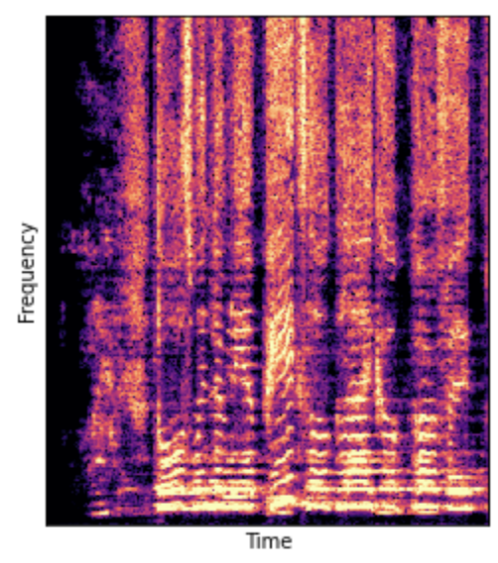
\includegraphics[width=0.6\textwidth]{research/dataset_preparation/PreprocessingSpecplot.png}
    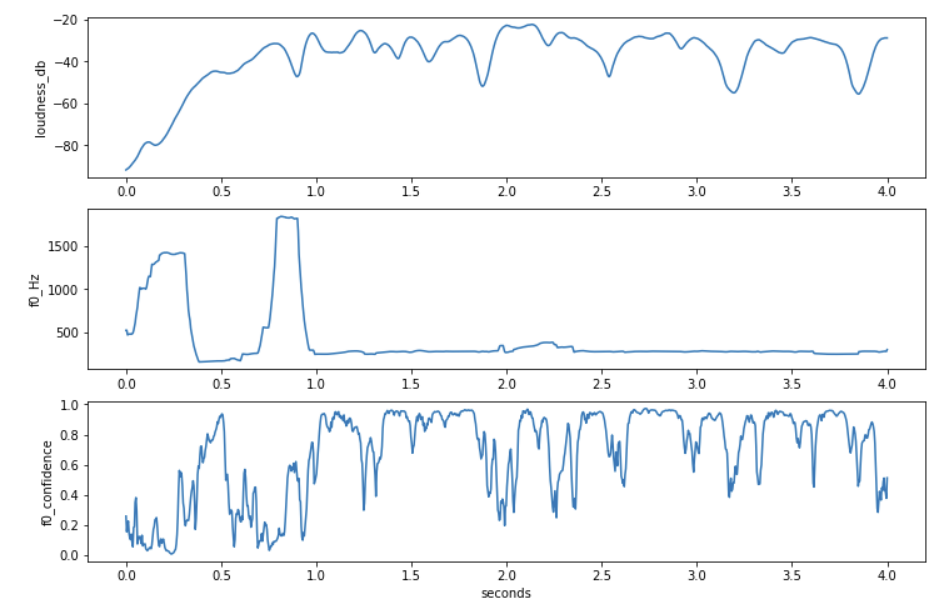
\includegraphics[width=0.8\textwidth]{research/dataset_preparation/PreprocessingFeatures.png}
    \caption{Dataset Pre-processing: Spectrogram plot of a random 4 second sample from one of the datasets and its accomanying F0, F0 Confidence and Amplitude characteristics over time throughout the sample}
\end{figure}

Pre-processing of the datasets involved spliting the raw audio into smaller samples each 4 seconds long. The sample length was limited to 4 seconds to avoid capturing too much information in one spectrogram that would make learning using the convolutional neural network difficult.

For each sample F0 and confidence of F0 probability was inferred using CREPE\cite{CREPE}. Amplitude was computed statistically using the Librosa library\cite{LibrosaPip}. Latent Z information was available through the the passing of the raw audio. The 4 second samples and accomanying features were then stored as TFRecord files.

Each of the 2 datasets were preprocessed on Google Colab notebooks, this process took approximately 40 minutes for each dataset using a NVIDIA Tesla V100 GPU.

Finally, from each dataset a random 4 second clip was selected to prove successful pre-processing. Its its spectrogram was computed and plotted. Computed F0, F0 Confidence and Amplitude characteristics were also plotted for the selected clip. The underlying audio sample could also be played.